\documentclass{article}
\usepackage{graphicx}
\usepackage{booktabs}
\usepackage{siunitx}
\usepackage[margin=1in]{geometry}
\usepackage[colorlinks=true, urlcolor=blue, linkcolor=black]{hyperref}

\title{Simulating the JV curve of a solar cell}
\author{Physics and Characterization of Emerging Solar Cells, UZH}
\date{October 2026}

\begin{document}

\maketitle

\section{Drift-diffusion simulator}

In this exercise we will use SIMsalabim\footnote{\url{https://github.com/kostergroup/SIMsalabim}},
an open-source drift-diffusion simulator for solar cells. We run it through its web interface at \url{http://simsalabim-online.com/}, so no installation is required. We will use the steady-state \textit{JV} simulator (Fig.~\ref{fig:jv}):

\begin{figure}[h]
    \centering
    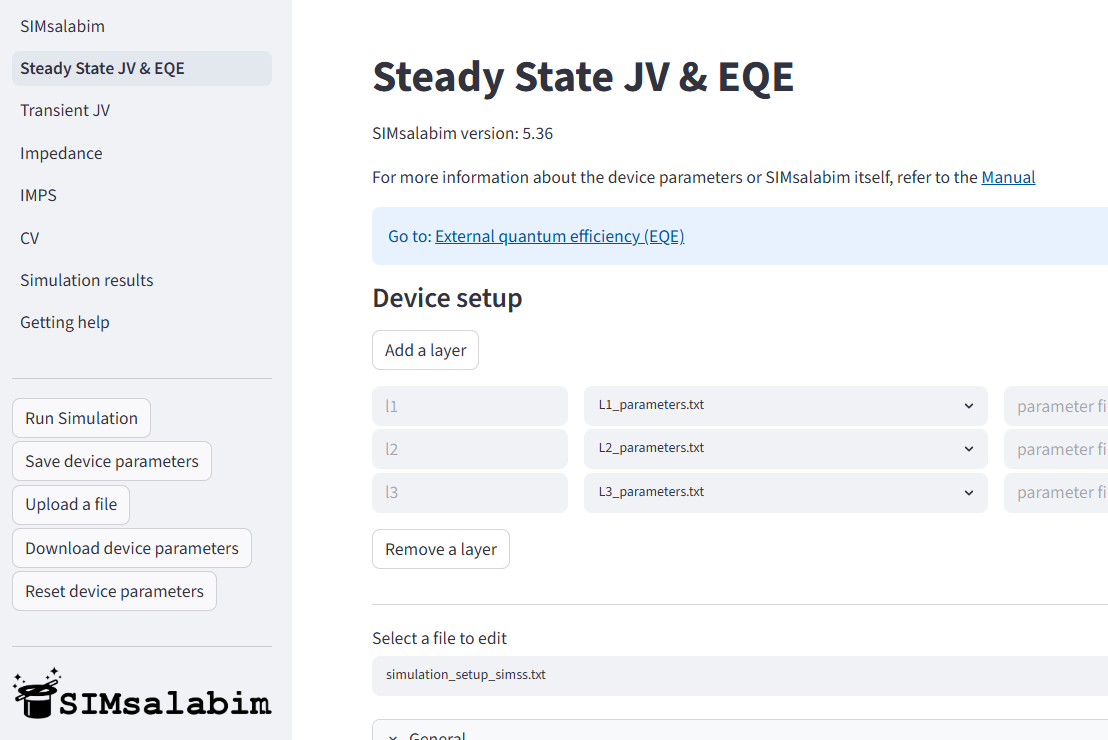
\includegraphics[width=\textwidth]{figures/jv.png}
    \caption{Online user interface of SIMsalabim steady-state \textit{JV} curve simulator.}
    \label{fig:jv}
\end{figure}

\section{Device model}

We model the solar cell as three semiconductor layers (Fig.~\ref{fig:devicediagram}): the absorber in the middle, where light is absorbed and electron--hole pairs are generated, sandwiched between two charge-selective transport layers, an electron transport layer (ETL) that lets electrons pass while blocking holes, and a hole transport layer (HTL) that does the opposite. For these simulations, only the absorber layer parameters will need to be modified.

\begin{figure}[t]
    \centering
    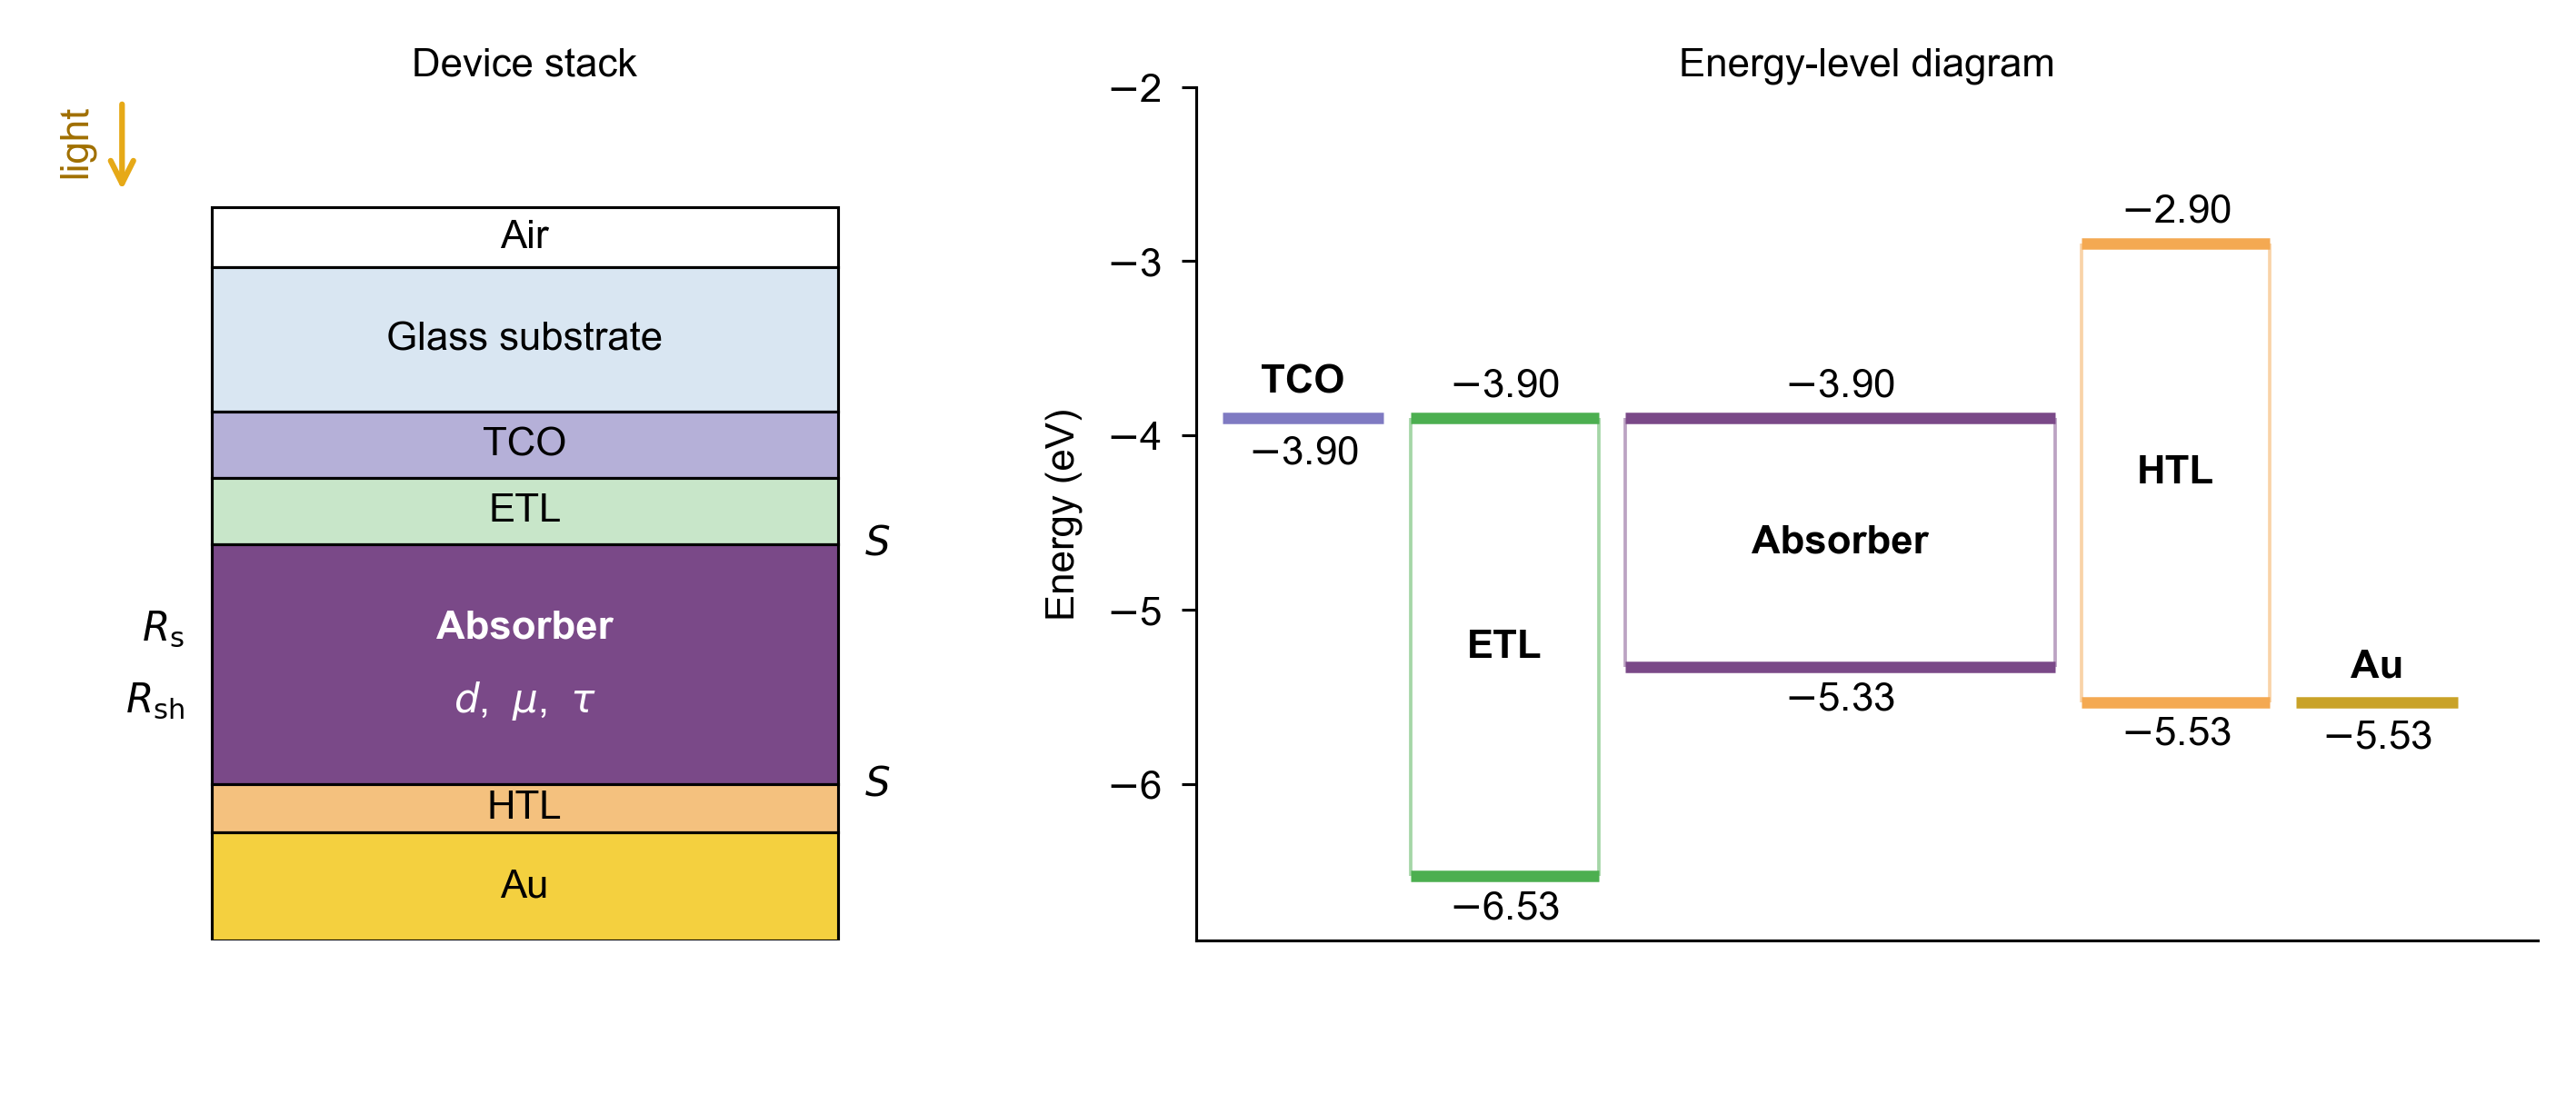
\includegraphics[width=\textwidth]{figures/00_stack_and_energy.png}
    \caption{Model device stack and energy-level diagram.}
    \label{fig:devicediagram}
\end{figure}

A simulation in SIMsalabim needs the simulation setup file and one parameter file per layer. For the absorber, we also will need to set the optical \texttt{nk} file. The rest of \texttt{nk} files for layers as well as the incident solar spectrum are already available in the online tool, so they do not need to be uploaded again. 

\paragraph{Download the starting input files.}
From the GitHub repository\footnote{\url{https://github.com/mtorrec/jv-simulations-simsalabim}}, download the \texttt{bad\_start/} folder. You should have:
\begin{itemize}
    \item \texttt{simulation\_setup.txt}
    \item \texttt{ETL\_parameters.txt}, \texttt{ABS\_parameters.txt}, \texttt{HTL\_parameters.txt}
    \item the \texttt{nk\_*.txt} files in \texttt{Data\_nk/} (only needed for absorber)
    \item the spectrum \texttt{AM15G.txt} in \texttt{Data\_spectrum/} (not needed)
\end{itemize}

\paragraph{Upload them to the GUI.}
In the right-hand menu (Fig.~\ref{fig:upload}, left), click \textbf{\textsf{Upload a file}}.
A dialog opens (Fig.~\ref{fig:upload}, right): select \textbf{\textsf{Simulation setup}} from
the dropdown, drop in \texttt{simulation\_setup.txt}, then upload the three layer parameter
files (\texttt{ETL/ABS/HTL\_parameters.txt}) under
\textbf{\textsf{Select all the layer parameter files\dots}} The dialog lists any
\textsf{Missing layer parameter files} until all three are in. Then click \textbf{\textsf{Submit}}. After doing this click on \textbf{\textsf{Save device parameters}} to update the model. Repeat the \textbf{\textsf{Upload a file}} step with the dropdown set to \textbf{\textsf{nk file}} to upload the absorber file \texttt{Data\_nk/nk\_absorber\_Eg1.43eV.txt} and again \textbf{\textsf{Save device parameters}}.

\section{Running the simulations}

\begin{figure}[h]
    \centering
    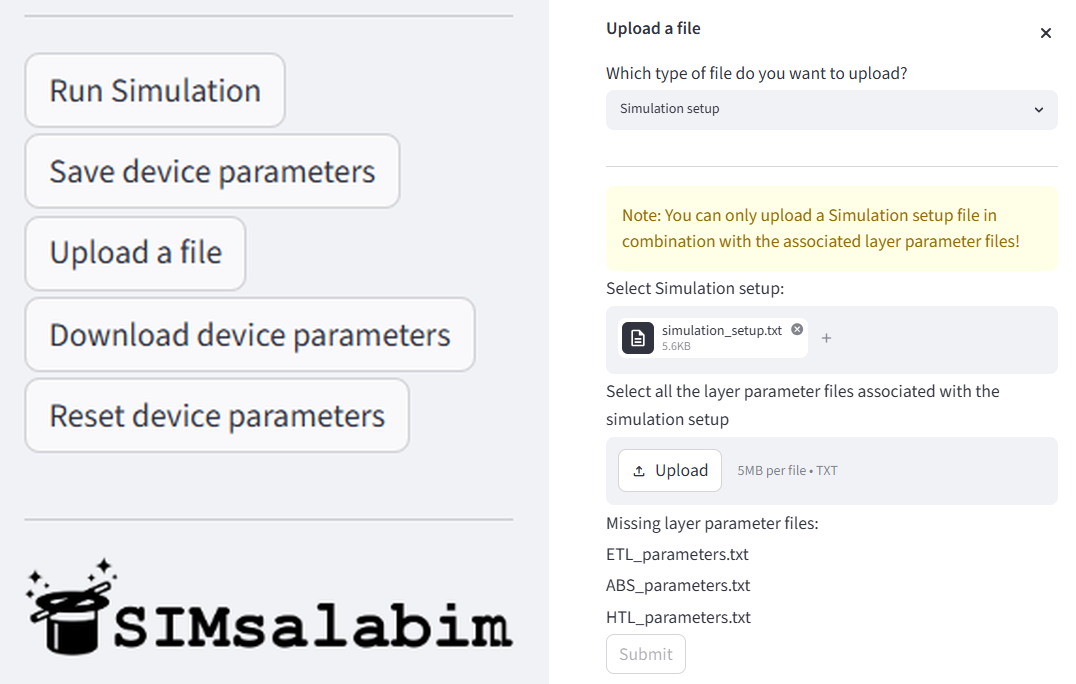
\includegraphics[width=0.9\textwidth]{figures/upload_combined.png}
    \caption{Uploading inputs. Left: side menu with the \textsf{Upload a file} button.
    Right: upload dialog --- pick the file type from the dropdown, then drag the files
    in. The \textsf{Missing layer parameter files} list disappears once all three
    layer files are uploaded.}
    \label{fig:upload}
\end{figure}

\paragraph{Run the simulation.}
Click on \textbf{\textsf{Run Simulation}} (top of the side menu, Fig.~\ref{fig:upload}, left). When the solver finishes, go to \textbf{\textsf{Simulation results}} in the main menu (Fig.~\ref{fig:jv}, left). The GUI should display the simulated \textit{JV} curve and the key figures of merit: $J_\mathrm{sc}$, $V_\mathrm{oc}$, FF, MPP. 

The obtained \textit{JV} should match the bad start in Fig.~\ref{fig:ref}. The parameters for the absorber in \texttt{bad\_start/}, listed in
Table~\ref{tab:absstart}, are not optimum for this solar cell.

\paragraph{Change parameters to improve the solar cell.}
Open \texttt{ABS\_parameters.txt} in the GUI's text editor (you can also edit the \texttt{.txt} file directly and re-upload each time). When using the GUI's editor (Fig.~\ref{fig:editfile}), after varying parameters always click on \textbf{\textsf{Save device parameters}} before running the simulation again. Modify the key absorber parameters, and check also the contact settings in the simulation setup file. The aim is to bring the device power conversion efficiency above 25\% (i.e., MPP above 250\,W\,m$^{-2}$), as close as possible to the target \textit{JV} curve in Fig.~\ref{fig:ref}.

\begin{figure}[h]
    \centering
    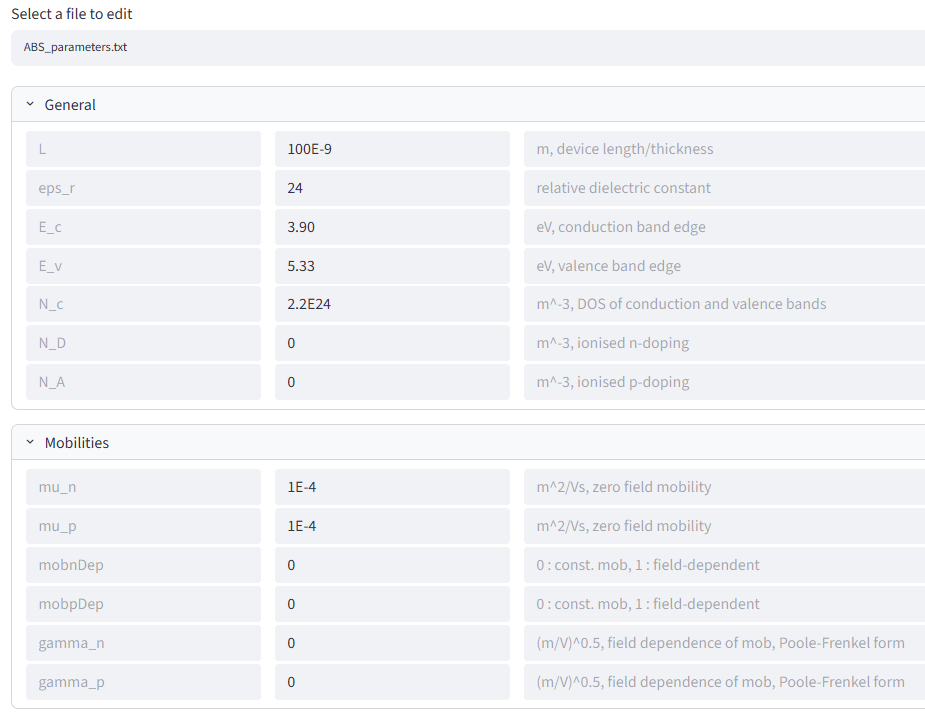
\includegraphics[width=\textwidth]{figures/editfile.png}
    \caption{Text editor of parameter and simulation setup files available in the GUI. To edit the simulation and layer parameters, change values in the text boxes and always click \textbf{\textsf{Save device parameters}} afterwards.}
    \label{fig:editfile}
\end{figure}

\begin{table}[h!]
    \centering
    \begin{tabular}{llll}
        \toprule
        Parameter & Symbol & Starting value & Unit \\
        \midrule
        Thickness                       & $L$              & $100$                & \si{nm}            \\
        Relative permittivity           & $\varepsilon_r$  & $24$                 & --                 \\
        Conduction-band edge            & $E_c$            & $3.90$               & \si{eV}            \\
        Valence-band edge               & $E_v$            & $5.33$               & \si{eV}            \\
        Effective DOS (CB and VB)       & $N_c$            & $2.2 \times 10^{24}$ & \si{m^{-3}}        \\
        Electron / hole mobility        & $\mu_n,\mu_p$    & $1 \times 10^{-4}$   & \si{m^2.V^{-1}.s^{-1}} \\
        Bulk trap density               & $N_{t,\mathrm{bulk}}$ & $2 \times 10^{22}$ & \si{m^{-3}}       \\
        Interface trap density (to HTL) & $N_{t,\mathrm{int}}$  & $5 \times 10^{15}$ & \si{m^{-2}}       \\
        Band-to-band recombination      & $k_\mathrm{direct}$   & $3 \times 10^{-17}$ & \si{m^3.s^{-1}} \\
        Optical absorption file         & \texttt{nkLayer} & \multicolumn{2}{l}{\texttt{nk\_absorber\_Eg1.43eV.txt}} \\
        \bottomrule
    \end{tabular}
    \caption{Starting values of the absorber parameters in \texttt{bad\_start/ABS\_parameters.txt}.
    The bandgap and band-edge alignments with the transport layers are already set; the other parameters are the ones that may need tuning.}
    \label{tab:absstart}
\end{table}

\begin{figure}[ht]
    \centering
    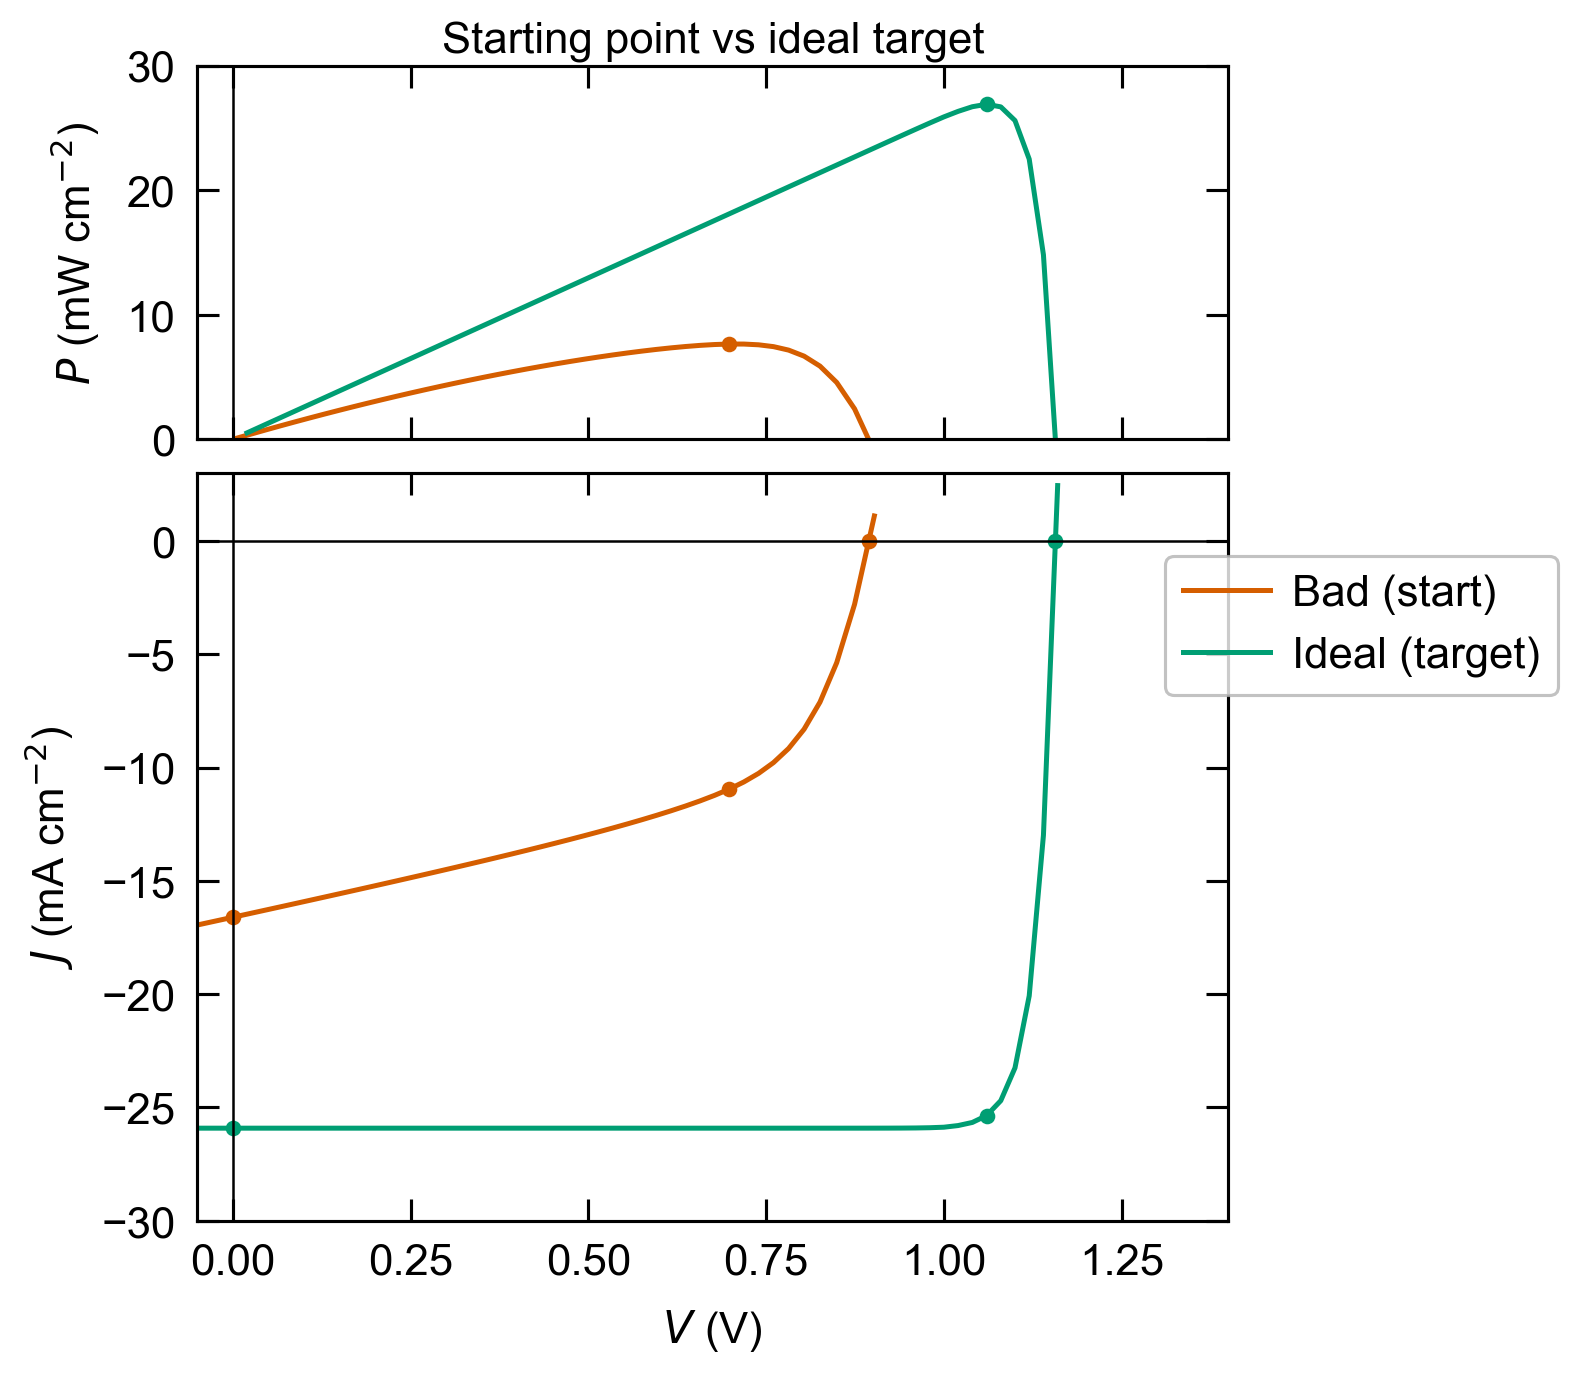
\includegraphics[width=0.75\textwidth]{figures/reference_JV.png}
    \caption{Starting point (orange) vs.\ ideal target (green).}
    \label{fig:ref}
\end{figure}

\end{document}
